\documentclass[letter,10pt]{article}
\usepackage[english]{babel}
\usepackage[utf8]{inputenc}
\usepackage{graphicx}
\usepackage{float}
\usepackage{amsmath,amsfonts,amssymb,mathtools,amsthm}
\usepackage{hyperref}
\graphicspath{ {./} }

%Includes "References" in the table of contents
\usepackage[nottoc]{tocbibind}

%Title, date an author of the document
\title{t-SNE: Theory and Methodology}
\author{Chenhui Zhang}

%Begining of the document
\begin{document}

\maketitle

\medskip

\section{Introduction}
In the paper \textit{Visualizing Data using t-SNE}\cite{vanDerMaaten2008}, Geoffrey Hinton and Laurens van der Maaten propose a new approach of dimensionality reduction, based on Hinton's previous work of SNE, through the stochastic search of lower dimension space to find a map that preserves the neighborhood structure of high dimensional data points. They first define a joint probability distribution $P$ in high-dimensional space given by the pair-wise similarities between high-dimensional data points calculated from applying Gaussian distribution centered around the data points to the square distance (or other similarity metrics) between a pair of points
$$
p_{ij}=\frac{\exp{(-\|\mathbf{x_i}-\mathbf{x_j}\|^2/2\sigma^2)}}{\sum_{k}\sum_{l\neq k}\exp(-\|\mathbf{x_k}-\mathbf{x_l}\|^{2}/2\sigma^2)}
$$
and a joint probability distribution $Q$ in low-dimensional space given by the pair-wise similarities between low-dimensional data points calculated from employing a Student t-distribution (for addressing the crowding problem) with one degree of freedom to the square distance (or other similarity metrics) between a pair of points
$$
q_{ij}=\frac{(1+\|\mathbf{\mathbf{y_i}-\mathbf{y_j}}\|^2)^{-1}}{\sum_{k}\sum_{l\neq k}(1+\|\mathbf{y_k}-\mathbf{y_l}\|^2)^{-1}}.
$$


However, in practice, $p_{ij}$ is defined, from the conditional probabilities to guarantee symmetry and address the problem of outliers, by
$$
p_{ij}=\frac{p_{i|j}+p_{j|i}}{2n}
$$
where
$$
p_{j|i}=\frac{\exp{(-\|\mathbf{x_i}-\mathbf{x_j}\|^2/2\sigma_i^2)}}{\sum_{k\neq i}\exp(-\|\mathbf{x_i}-\mathbf{x_k}\|^{2}/2\sigma_{i}^2)}.
$$
Finally, Kullback-Leibler divergence is introduced to measure the similarity between $P$ and $Q$. In this case, it is cross-entropy function, off by one negative sign, given by
$$
C=KL(P||Q)=\sum_{i}\sum_{j}p_{ij}\log{\frac{p_{ij}}{q_{ij}}}.
$$
Since this function punishes mapping neighbors (larger $p_{ij}$) to widely separated points (small $q_{ij}$), Hinton and Laurens define this as the loss function to optimize with gradient descent with momentum.

\section{Novelty}

Although the main idea of t-SNE had already been laid out by Hinton in 2002 before this paper was published, this paper still presents a lot of improvements on the original paper.

For example, t-SNE employs a Student's t-distribution with degree of freedom $1$ to calculate the pair-wise similarity in low-dimensional map. In order to justify this modification, we need to get back to the reason why the crowding problem happens at the first place. Let's first consider a simple case: imagine we have four points in $\mathbb{R}^4$ that are equidistant to each other and now we want to map them to the points in $\mathbb{R}^3$ in a way such that they are also equidistant (i.e. preserving neighborhood structure defined by distance metric). However, this is simply impossible without squishing two points into one point. If we generalize this situation into high dimensional manifolds, the same problem will only get worse: there is not enough area in the low-dimensional map to accommodate moderately distant data points! The author uses an analogy to the interactions of an N-body system to further explain this problem from the gradient of its loss function. If two nearby points are mapped far away, then their will be a high attractive force (high gradient) that pull the points back together; if the two points are already very far away originally, the attractive force will be very weak whatsoever. However, following this logic, the attractive force on a data point is also related to the number of data points that exert the force. Albeit the weak attraction per data point, "the large number of such forces crushes together the points in the center of the map," leading to the crowding problem. t-SNE approaches this problem in a more natural way by converting distance into symmetric joint probabilities, one under Gaussian distribution and the other under Student's t-distribution. Let's consider again two data points that are far away. It's no doubt that they will have very small $p_{ij}$ but this time they will have even bigger $q_{ij}$, compared with its counterpart in vanilla SNE, since the tail of a Student-t distribution is very heavy compared with that of a Gaussian distribution. If we plug $p_{ij}$ and $q_{ij}$ back into the KL divergence in t-SNE, we will have a smaller value than that in SNE. Hence, the attractive force between far away points will be smaller so that the probability of points being crushed together is reduced and the attractive force. From a more probabilistic perspective, Student's t-distribution will make $q_{ij}$ more prone to falling far from the mean and result in the increase of similarity between $p_{ij}$ and $q_{ij}$ for far away points so that they won't be punished too much for being apart.

Laurens and Hinton also brought the trick of "early compression" and "early exaggeration" into the optimization methods for t-SNE. The sum of the squared distance of the mapped points from the origin is introduced into the loss function in early stage of training so that the map points will be forced to stay together at the start, resulting in the convenience of clustering. They also "exaggerate" the calculated $p_{ij}$'s by a certain factor so that the $q_{ij}$'s will be too small to model $p_{ij}$'s. The authors claim that this maneuver will create a lot of relatively empty space on the map so it will be easier to move data points later. However, I have doubt on whether these approaches will help solve the overcrowding problem so the trade-off of making such decision needs further justification. In addition, I find justifying problems with analogies in physics not convincing enough, albeit being intuitive.

t-SNE also addresses the problem of using the Euclidian distance as similarity metric by using a probability distribution and preserving small pair-wise distance instead: if the dataset lies in a high-dimensional non-linear manifold, the Euclidian distance may not truly represent the similarity. In the example below, the two data points on the two-dimensional manifold are close to each other in terms of the Euclidian distance, but they are far from similar in terms of the overall structure. 

\begin{figure}[H]
    \centering
    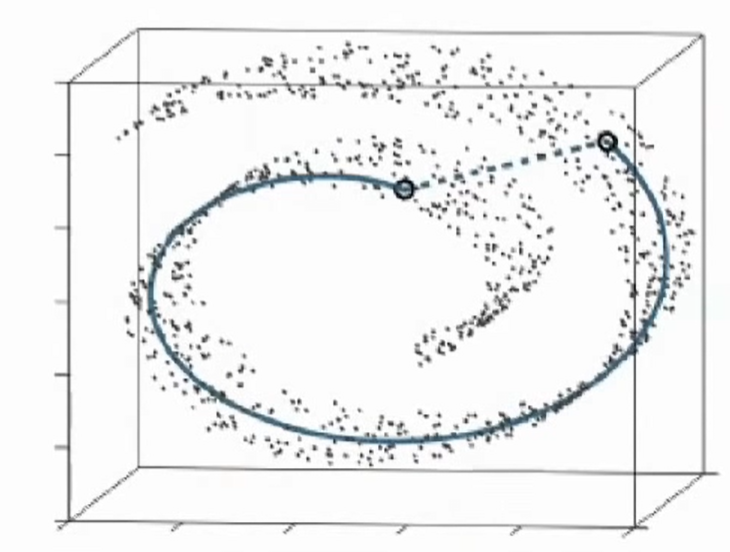
\includegraphics[scale=0.5]{pca_limitation}
    \caption{PCA's Limitation on Non-linear Data}
    \label{fig:pca_limitation}
\end{figure}

\pagebreak
In general, t-SNE works exceptionally well in visualizing non-linear data since it preserves the local structure of the dataset. Let's compare it with "traditional" linear dimensionality reduction method PCA, which preserves the large variance and pair-wise distance in the data. For example, if we run PCA on the MNIST dataset and keep the first two PCs, we can clearly see the very large variance along the two PCs ($1$ and $0$ are very different in their shape). However, the local structure is not well preserved for more similar digits.

\begin{figure}[H]
    \centering
    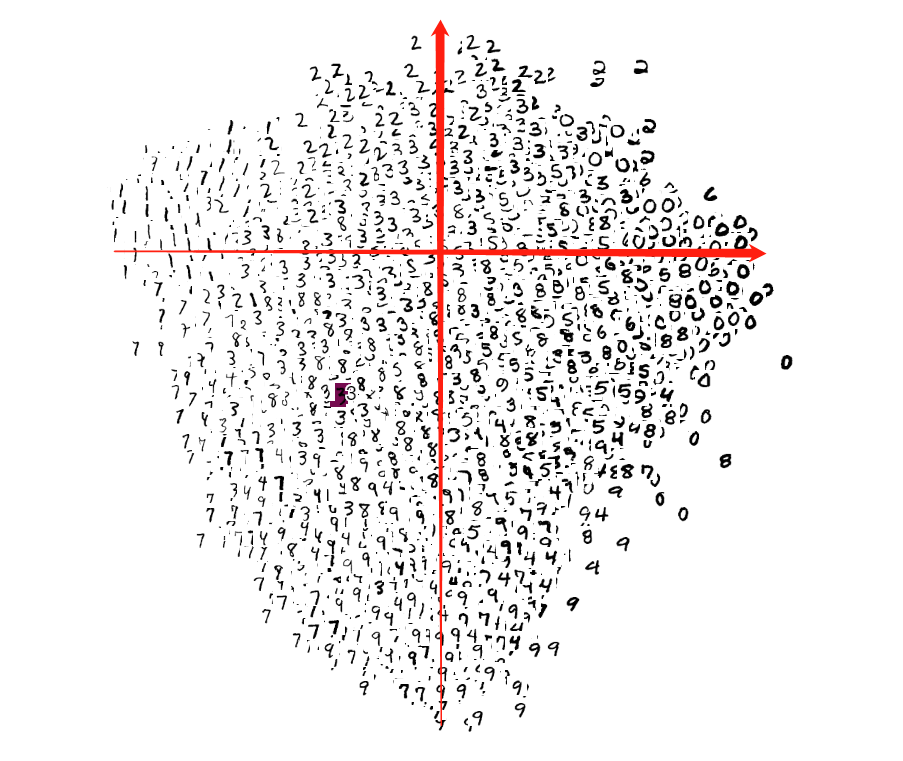
\includegraphics[scale=0.5]{mnist_pca.png}
    \caption{PCA on MNIST}
    \label{fig:pca_mnist}
\end{figure}

\pagebreak
t-SNE, on the other hand, clearly shows the preservation of local structure like the clustering in the higher dimension. However, coordinate axes don't make any sense here since it's non-linear and can't quite give us some "principal components."

\begin{figure}[H]
    \centering
    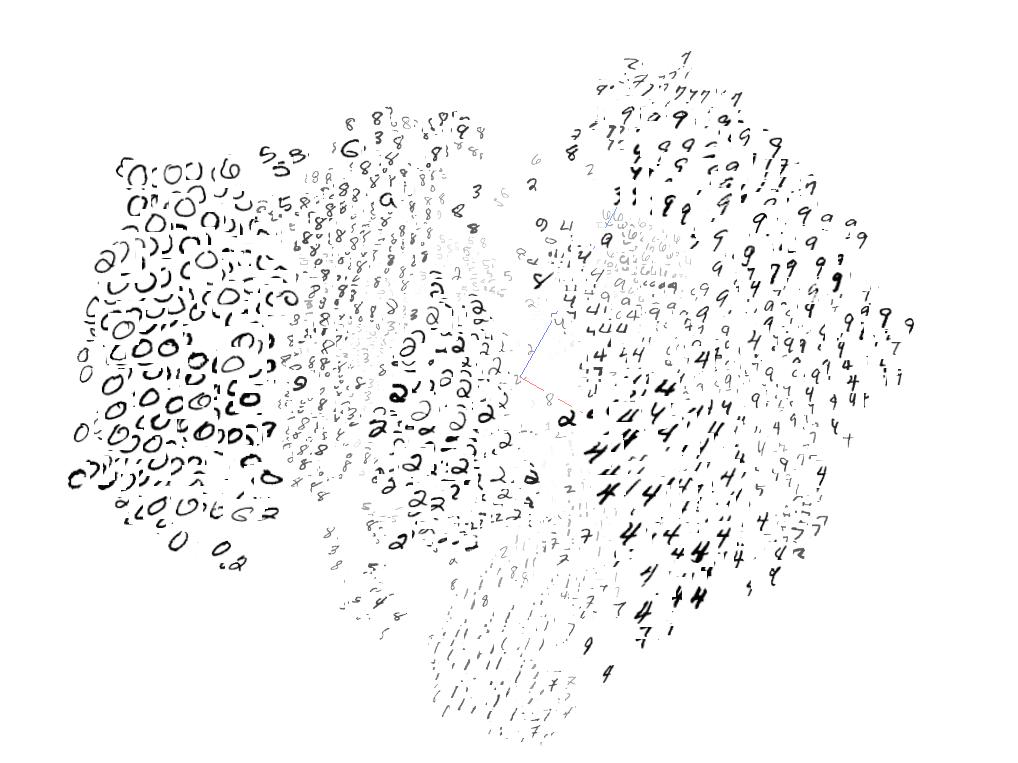
\includegraphics[scale=0.5]{mnist_tsne.png}
    \caption{t-SNE on MNIST}
    \label{fig:tsne_mnist}
\end{figure}

t-SNE also comes with some limitations. For example, the original paper uses a single map. This may be particularly awkward when we are trying to visualize word embeddings with a single map based on the semantic similarities. As pointed out by Laurens in one of his tech talks\cite{Maaten13:online}, the word "river" has semantic similarity with the word "bank" and the word "bank" is also similar to the word "bailout". Therefore, in a single map, "river" will be mapped as a neighbor of "bailout" by triangle inequality. However, the "similarity" between "river" and "bailout" doesn't make sense at all. Hinton and Laurens also point some other weakness of t-SNE at the end of the paper. First, they have doubt about t-SNE's ability of generalization. t-SNE performs exceptionally well on the task of data visualization (i.e. reducing dimensionality to two or three) because of its mitigation of crowding problem and the delicate choice of Student's t-distribution. However, it is also the behavior of Student's t-distribution of degree of freedom $1$ make the authors have doubt about the readiness of t-SNE for reducing high dimensional data to a dimension that is greater than $3$. Indeed, since this algorithm is equivalent to the search of lower dimension space for a optimal map of data points in higher dimension, the No Free Lunch Theorem tells us that if it's highly specialized on reducing dimension to less than or equal to three, then it may have problem in serving more general purpose. Second, this algorithm may be daunted with the curse of intrinsic dimensionality since manifold learning algorithm implicitly assumes local linearity and this rule may be violated in datasets with a high intrinsic dimensionality. Third, compared with the state of art techniques in dimensionality reduction, t-SNE has a non-convex loss function. However, the authors claim that this is insufficient to reject t-SNE as a visualization method.

\section{Improvement}

In Laurens' later paper \textit{Accelerating t-SNE using Tree-Based Algorithms}\cite{journals/jmlr/Maaten14}, he introduced the Barnes-Hut Approximation of the t-SNE gradient. The Barnes-Hut Approximation was first used to approximate the force exerted by stars. Here, the intuition is the same. Since the "forces" exerted by the members in a group of nearby data points on a data point that is far away are roughly the same, the Barnes-Hut Approximation treat those nearby points as one point in the "center of mass" and calculate the force from that point, assigning that result to all the nearby points. This method reduces the time-complexity of calculating gradients to $O(n\log n)$.

Since the authors mentioned that the non-convexity of the loss function constitutes one of the major weakness of t-SNE, maybe it's also possible to improve the convergence speed with Adam. It's understandable that Hinton and Laurens used SGD with momentum since Adam came out as a conference at ICLR 2015 but it looks like nobody (at least from published papers) has formally experimented with using Adam to optimize the loss function of t-SNE.

\section{Experience}

This assignment not only serves as my introduction to t-SNE, but also provides a survey on the popular dimensionality reduction methods and their advantages and limitations. Besides, I've also learned more about the theories for evaluating a learning model, especially the Free Lunch Theorem and the analysis  inductive bias.

This assignment definitely strengthened my understanding about the knowledge in class, especially about probability distributions.

Besides, I'm also surprised by how machine learning problems can be interpreted as physics problem from which we can gain more intuition.

\medskip

%Sets the bibliography style to UNSRT and imports the 
%bibliography file "samples.bib".
\bibliographystyle{unsrt}
\bibliography{citation}

\end{document}
